\chapter{Tworzenie oprogramowania}
\label{cha:tworzenie_oprogramowania}

\section{Opis użytej technologii i bibliotek}

Aplikacja serwerowa została stworzona w opisanym we wcześniejszych paragrafach środowisku Node.js. W celu przyspieszenia procesu tworzenia kodu korzysta z wielu zewnętrznych bbibliotek open-source. Standardowym oprogramowaniem służącym do zarządzania zewnętrznymi bibliotekami jest aplikacja \textit{npm}, jednak podczas tworzenia projektu użyto aplikacji \textit{yarn}, Działa ona w bardzo przybliżony sposób, zabezpiecza jednak przed usunięciem przez twórcę kodu źródłowego oprogramowania każdej z bibliotek. W poniższych punktach opisano kilka wybranych bibliotek użytych do stworzenia aplikacji wraz z krótkim opisem i przykładem użycia:\newline

\textbf{Express} - biblioteka służąca do pisania aplikacji serwerowych przy użyciu biblioteki Node.js. Udostępnia prosty interfejs do tworzenia punktów końcowych i jest określana jako jeden ze standardów podczas tworzenia aplikacji serwerowych przy użyciu Node.\newline

\textbf{Eslint} - biblioteka służąca jako tzw. \textit{linter}, czyli proces na bieżąco sprawdzający jakość kodu pisanego przez użytkownika. Dzięki użyciu eslint programista nie musi martwić się o niejednorodność we wcięciach, nieużywane zmienne czy niepoprawne ilości znaków białych, jest to sprawdzane przez program. Eslint korzysta z pliku .eslintrc który definiuje wszystkie zasady które mają być spełnione w projekcie, aby kod został uznany za bezbłędny.\newline

\textbf{Axios} - biblioteka umożliwiająca proste interakcje z interfejsami serwerowymi innych serwisów. Dzięki stworzeniu globalnego klienta axios zawierającego podstawową konfigurację, nie ma potrzeby powielać tych samych konfiguracji w wielu zapytaniach, wystarczy jedynie zdefiniować rzeczy, które się różnią, jak na przykład URL czy metoda HTTP.\newline

\textbf{Cors} - w celu komunikacji aplikacji serwerowej i strony internetowej znajdujących się pod jednym adresem IP należy skonfigurować \textit{„Cross Origin Resource Sharing”}. Ma to zapobiec możliwości przesyłania złośliwych skryptów w formularzach, które zostaną wykonane przez aplikację. Do umożliwienia Cross Origin Resource Sharing użyto biblioteki cors, która po inicjalizacji automatycznie dodaje nagłówek HTTP Access-Control-Allow-Origin z odpowiednią domeną, dla której tego typu zapytania mają być możliwe.\newline

Aplikacja w celu wyznaczania tras korzysta z dwóch zewnętrznych serwisów - ZiKIT Carto oraz openstreetmap. Carto jest to platforma do zarządzania danymi geoprzestrzennymi, która umożliwia pobranie, wizualizację oraz przeszukiwanie dróg przy użyciu odpowiednich komend SQL. Kod Carto jest otwarty i każdy może uruchomić go w swojej stronie internetowej w celu uproszczonej wizualizacji tras na mapie. Krakowski ZiKIT korzysta z własnej instancji Carto w celu wizualizacji i przetrzymywania wszelkiego rodzaju danych, takich jak zbiory różnych typów dróg oraz wydarzenia (np. wypadki samochodowe) na mapach.\newline 
Openstreetmap jest to darmowy portal udostępniający usługę map oraz oferujący szeroki zakres innych danych geoprzestrzennych. Openstreetmap jest projektem otwartym, portal jest utrzymywany przez fundację o tej samej nazwie, a swoje dane zawdzięcza użytkownikom, którzy wprowadzają je w celu ich późniejszego wykorzystania lub jako wolontariusze.

\subsection{Opis udostępnionych endpointów}

W celu umożliwienia komunikacji aplikacji mobilnej oraz strony internetowej, przygotowana aplikacja serwerowa udostępnia pod zdefiniowanymi adresami URL end-point’y, które po przekazaniu odpowiednich parametrów w kwerendzie, umożliwiają pobranie danych. Zaimplementowano je przy pomocy obiektu \textit{router}, będącego częścią opisanej wcześniej biblioteki express.
Poniżej przedstawiono dwa end-point’y udostępnione przez aplikację razem z dokumentacją oraz przykładową, skróconą, odpowiedzią w formacie JSON:
\begin{enumerate}
\item Endpoint findOptimized

Używany przez aplikację mobilną w celu pobrania optymalnej trasy pomiędzy dwoma punktami przekazanymi w formie kwerendy. Wykorzystuje metodę HTTP GET. Możliwe parametry do przekazania w kwerendzie URL:

\begin{itemize}
\item startLocation - parametr określający punkt początkowy wyznaczonej trasy w przypadku, gdy jest on przekazany jako adres.
\item startLocationLatitude oraz startLocationLongitude - przez te parametry zostaje przekazana pozycja użytkownika w przypadku, gdy zostaje ona zdefiniowana przez współrzędne geograficzne punktu początkowego. Jeśli lokalizacja punktu początkowego zostaje przekazana w tej postaci, parametr startLocation zostaje zignorowany, niezależnie od tego czy został zdefiniowany w kwerendzie.
\item endLocation - parametr określający punkt końcowy trasy w postaci adresu. Aplikacja nie daje możliwości przekazania punktu końcowego trasy w postaci współrzędnych geograficznych, dlatego też w przypadku punktu końcowego trasy przekazanie lokalizacji w tej postaci nie zostało zaimplementowane.
\item routeType - określenie czy wyznaczona trasa ma być najkrótsza, czy optymalna z wagowego punktu widzenia. Przyjmuje parametr typu String o wartość BEST lub SHORTEST. W przypadku braku, brana jest domyślna wartość BEST.
BEST lub SHORTEST.
\item algorithm - parametr określający jaki algorytm ma zostać użyty do wyszukania trasy. Przyjmuje parametr typu String o wartości ASTAR, AGREEDY lub NBA. W przypadku braku parametru, aplikacja używa algorytmu NBA.
\end{itemize}

Przykładowe zapytanie HTTP GET w celu uzyskania odpowiedzi zawierającej optymalną trasę przejazdu można uzyskać pod adresem URL:

\url{bazowy_adres_url/api/routes/findOptimized?startLocation=romera&endLocation=karmelicka&routeType=BEST}

Przykładową odpowiedź, skróconą do postaci przedstawiającej jej formę przedstawiono poniżej.

\begin{figure}[H]
\centering
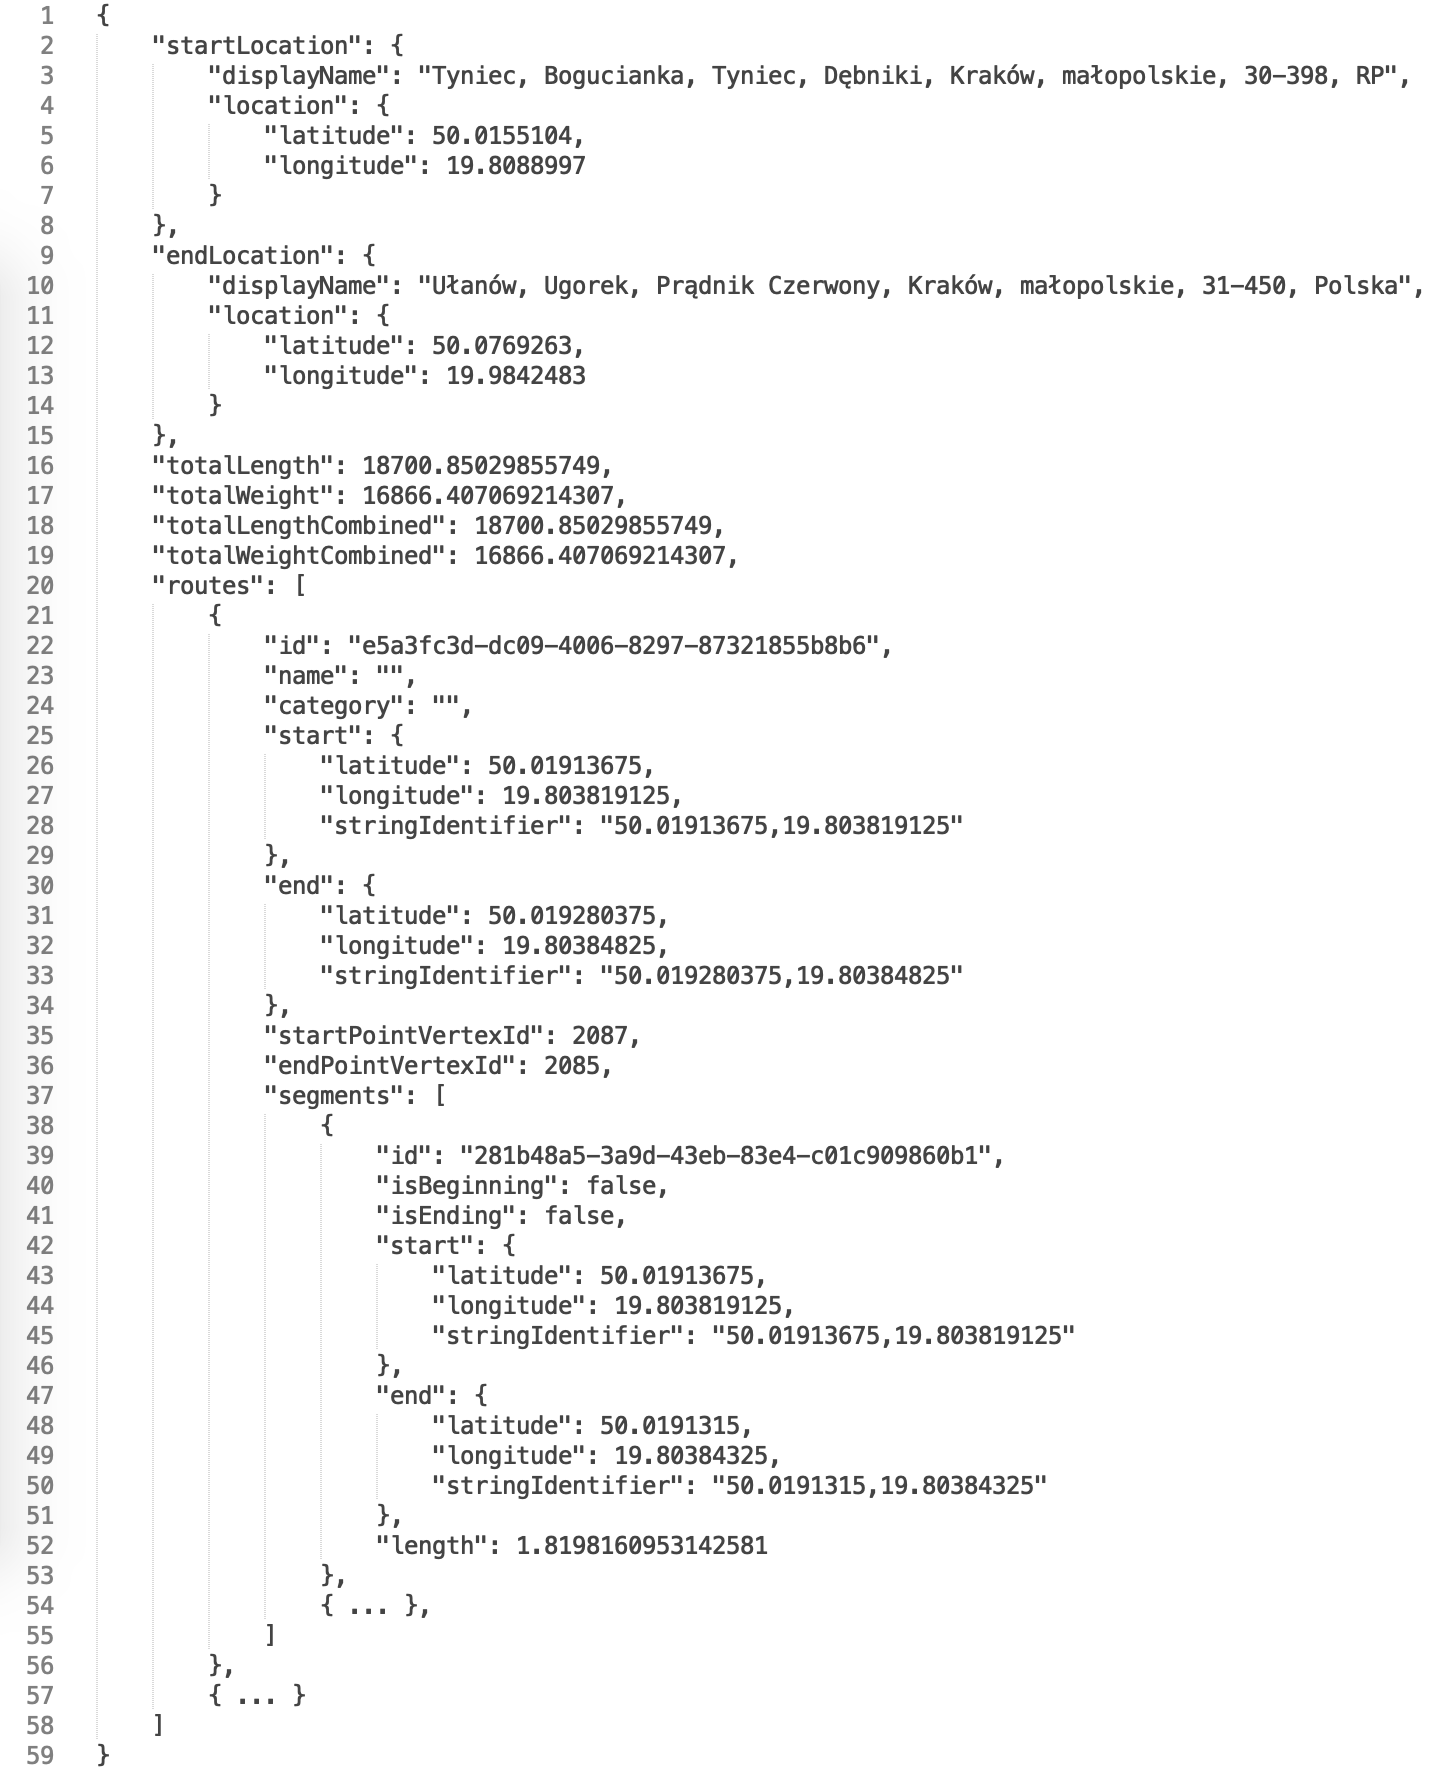
\includegraphics[height=12cm]{api_response_json}
\caption{Przykładowa odpowiedź na zapytanie serwera pod endpoint findOptimized.}
\end{figure}

\item Endpoint visualizationPoints:

Używany przez stronę internetową, będącą częścią przygotowanego systemu, w celu wizualizacji trasy na mapach openstreetmap. Wykorzystuje metodę HTTP GET. Możliwe parametry do przekazania w kwerendzie URL:

\begin{itemize}
\item startLocation - parametr określający początkową lokalizację użytkownika w postaci adresu.
\item endLocation - parametr określający końcową lokalizację użytkownika w postaci adresu.
\item routeType - określenie czy wyznaczona trasa ma być najkrótsza, czy optymalna z wagowego punktu widzenia. Przyjmuje parametr typu String o wartości BEST lub SHORTEST.
\item algorithm - parametr określający jaki algorytm ma zostać użyty do wyszukania trasy. Przyjmuje parametr typu String o wartości ASTAR, AGREEDY lub NBA. W przypadku braku parametru, aplikacja używa algorytmu NBA.
\end{itemize}

Przykładowe zapytanie HTTP GET w celu uzyskania odpowiedzi zawierającej optymalną trasę przejazdu można uzyskać pod adresem URL:

\url{bazowy_adres_url/api/routes/visualizationPoints?startLocation=romera&endLocation=karmelicka&routeType=BEST&algorithm=ASTAR}

Przykładową odpowiedź, skróconą do postaci przedstawiającej jej formę przedstawiono poniżej:

\begin{figure}[H]
\centering
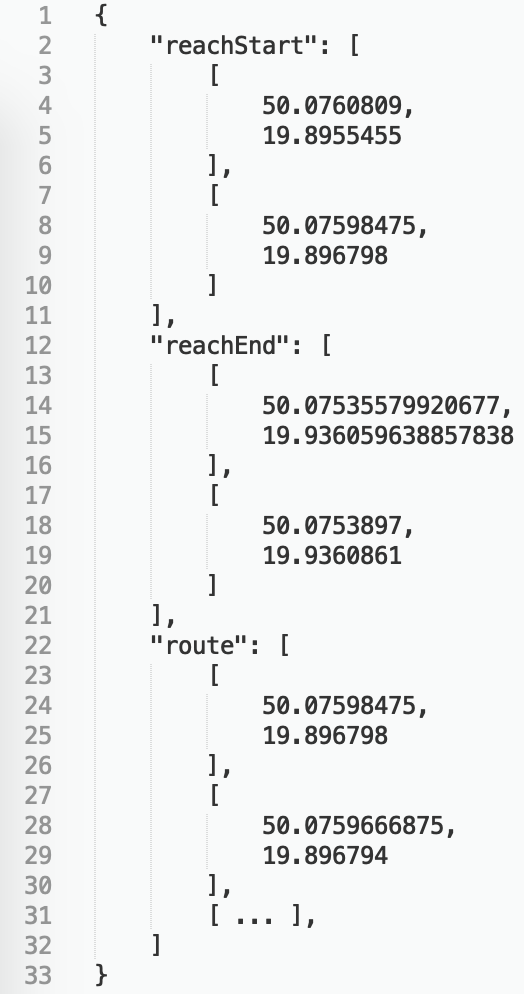
\includegraphics[height=12cm]{api_response_viz_json}
\caption{Przykładowa odpowiedź na zapytanie serwera pod endpoint visualizationPoints.}
\end{figure}

\end{enumerate}

\subsection{Proces wyznaczania grafu na podstawie pobranych danych}

W celu dodatkowej wizualizacji na poniższym schemacie blokowym przedstawiono proces wyznaczania grafu na podstawie pobranych danych geoprzestrzennych:

\begin{figure}[H]
\centering
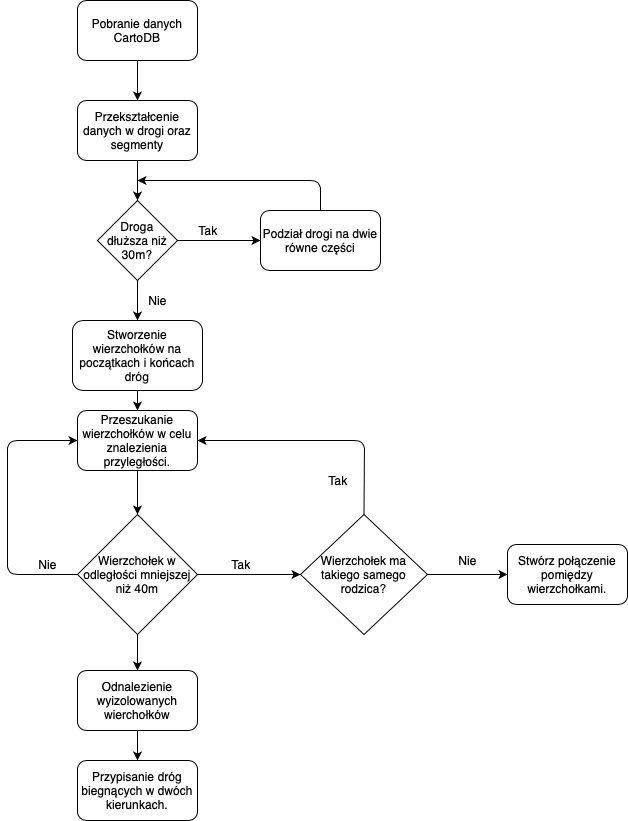
\includegraphics[height=16cm]{algorytm_schemat_blokowy}
\caption{Schemat blokowy algorytmu użytego do stworzenia grafu na podstawie danych geoprzestrzennych.}
\end{figure}

W celu optymalizacji czasu działania systemu, dane geoprzestrzenne są pobierane oraz przetwarzane przez aplikację tylko jeden raz, zaraz po włączeniu. Jest to czasochłonny proces, wymagający wielu iteracji po rozległym zbiorze danych. Jego rezultatem jest stworzenie grafu, który może być w kolejnych etapach wykorzystywany jako gotowa dana wejściowa. Tworzenie grafu zostaje rozpoczęte przez pobranie zestawu danych geoprzestrzennych dla miasta Kraków z portalu \textit{https://zikit.carto.com}. Pobrana baza danych zawiera zarówno trasy rowerowe, jak i drogi z ograniczeniem prędkości poniżej 50 kilometrów na godzinę, obydwie bazy są następnie scalane i przekształcane w zbiór odpowiednich dróg i segmentów. Droga jest logiczną reprezentacją krzywej poprowadzonej na mapie pomiędzy dwoma punktami, składa się z segmentów, które zawierają jedynie punkt początkowy oraz końcowy i definiują zestaw linii prostych, które mogą zostać użyte, aby narysować linię drogi na mapie. Wykorzystując metodę Haversine, zostają wyznaczone długości każdej drogi przez zsumowanie długości wszystkich segmentów, które się na nią składają. \newline
Kolejnym etapem jest proces przygotowywania dróg do procesu tworzenia grafu. Aby mieć pewność, że wszystkie przyległości zostaną poprawnie odnalezione, w pierwszym kroku należy odpowiednio podzielić wszystkie pobrane drogi na takie o mniejszej długości. Trasy pobrane z serwisu Carto mają bardzo losowe długości oraz są zaznaczone w taki sposób, że nie występuje segmentacja w okolicach końców innych tras oraz przy przecięciach z nimi. Z tego powodu wyznaczenie poprawnego grafu z uzyskanych danych wymaga wcześniejszego przetworzenia. Pierwszym krokiem przetwarzania danych jest podzielenie segmentów uzyskanych z przeanalizowanych, pobranych danych na takie, które mają maksymalnie trzy metry długości. Dzieje się to przez podział każdego segmentu na pół do momentu aż osiągną one pożądaną długość. W następnej kolejności, gdy posiadamy już podzielone segmenty, następuje podzielenie tras. Dzieje się to na zasadzie podzielenia tablicy segmentów na części o określonej długości a następnie utworzenia zestawu nowych dróg z uzyskanych części. Każda droga, stworzona przez podzielenie innej drogi na mniejsze części, posiada także przypisanie swojego "rodzica", czyli pierwotnej drogi z której nastąpił podział. Droga, będąca "rodzicem", posiada za to tablicę zawierająca wszystkie drogi będące jej "dziećmi". Na tym etapie następuje także przypisanie drodze odpowiedniej wagi oraz stwierdzenie czy droga przebiega po moście - jest to stwierdzane na podstawie wykrycia słów kluczowych „most” lub „kladka” w nazwie trasy. Niestety baza danych Carto ZiKiT nie oferuje w swoich danych takich informacji, dlatego też występuje potrzeba przewidzenia tej danej w inny sposób. \newline
Proces tworzenia grafu rozpoczyna się od stworzenia wierzchołka w każdym miejscu będącym zakończeniem lub rozpoczęciem drogi. W tym celu następuje iteracja po wszystkich drogach będących "rodzicami", dla każdej z nich następuje iteracja po wszystkich jej "dzieciach" i tworzone są wierzchołki na początku pierwszej drogi oraz na zakończeniu każdej następnej. Każdy z utworzonych w tym procesie wierzchołków ma także przypisywaną trasę "rodzica", który jest "rodzicem" drogi, dla której wierzchołek został stworzony. Kolejnym etapem jest wyszukanie przyległości dla każdego z wierzchołków. W tym celu następuje zagnieżdżona iteracja po wszystkich stworzonych wierzchołkach i porównywana jest odległość pomiędzy nimi. W przypadku, gdy odległość ta jest mniejsza niż 40 metrów, następuje połączenie wierzchołków drogą o typie \textit{standard link}. W tym procesie ignorowane są wierzchołki posiadające takiego samego "rodzica", w celu uniknięcia łączenia wierzchołków już ze sobą połączonych w obrębie jednej drogi. Ignorowane są także wierzchołki których trasa-rodzic znajduje się na moście, wyodrębniając z tego wyjątek, gdy aktualnie rozpatrywany wierzchołek jest początkiem lub końcem trasy, do której przynależy. Zabieg ten ma na celu uniknięcie łączenia za sobą dróg znajdujących się na różnej wysokości.
W kolejnym kroku działania algorytmu, obsługiwane są drogi dwukierunkowe, są to takie które w polu kategoria zawierają jeden z poniższych skrótów:

\begin{itemize}
\item dwr - droga rowerowa.
\item cpr - ciąg pieszo-rowerowy.
\item c16t22 - chodnik z dopuszczonym ruchem rowerowym (skrót pochodzi od identyfikatora znaku drogowego).
\item kontrapas i kontraruch - zakładamy, że w tym przypadku użytkownik może poruszać się w przeciwną stronę po ulicy, na której znajduje się dana ścieżka.
\item skróty pokrewne zawierające kombinację powyższych lub dopisek w postaci cyfry.
\end{itemize}

Każda z dróg przypisanych do każdego z wierzchołków, w przypadku gdy jest oznaczona jako dwukierunkowa, musi zostać odpowiednio przetworzona, aby algorytm wyszukiwania mógł przez nią prowadzić. W tym celu wszystkie takie drogi wychodzące z wierzchołka zostają dodane do dróg wchodzących do wierzchołka, a następnie zostają odwrócone, czyli podmieniany jest identyfikator wierzchołka początkowego oraz końcowego, współrzędne końca i początku, a także w analogiczny sposób zostaje odwrócony każdy segment przynależący do danej drogi. Ta sama procedura zostaje powtórzona w celu transformacji także dróg wchodzących do wierzchołka.
Ostatnim z kroków przygotowywania grafu jest wyodrębnienie samotnych wierzchołków. Są to wierzchołki, które znajdują się w mało zagęszczonym drogami obszarze i znajdują się zbyt daleko, aby znaleźć dla nich przyległości, pomimo że powinny one zostać znalezione. Przykładem dla tego przypadku może być droga rowerowa na mało uczęszczanej ulicy, która w pewnym momencie z braku możliwości poprowadzenia zostaje przerwana na odcinku długości 100-150m, po czym następuje jej kontynuacja w obrębie tej samej ulicy. W tym celu dla każdego z wierzchołków, który posiada tylko jedną drogę przychodzącą, zostaje przeszukana okolica najbliższych 150 metrów. W przypadku znalezienia zbyt dużej ilości przyległości, proces jest ignorowany. W przeciwnym wypadku wierzchołek zostaje z nimi połączony drogą typu \textit{isolation link}. \newline

Po przeprowadzaniu całego powyższego procesu zostaje wygenerowany graf składający się z wierzchołków, w którym drogi pełnią rolę krawędzi. Ostatnim krokiem, przeprowadzanym podczas tworzenia docelowego grafu, jest przypisanie wagi każdej z dróg. Zważając na fakt, że baza danych carto zawiera informacje odnośnie typów większości tras, aplikacja stara się przewidzieć zysk użytkownika z przebycia dłuższego dystansu znacznie bardziej komfortowymi drogami. W tym celu przypisywane są w zależności od kategorii wagi:

\begin{itemize}
\item Ddr - waga 0.7
\item Cpr - waga 0.8
\item Kontrapas, kontraruch - waga 0.8
\item C16t22 - waga 0.9
\item Standard link - w przypadku, gdy krótszy niż 10 metrów, posiada wagę 1.5. W przeciwnym wypadku waga jest równa 2.
\item Isolatation link - waga 4
\item Droga rowerowa bez kategorii - waga 1
\item Droga z bazy sugerowanych tras - waga 1.2
\end{itemize}

\subsection{Opis procesu wyznaczania trasy dla użytkownika}

Kolejnym etapem działania algorytmu jest wyszukiwanie tras na podstawie danych wejściowych przekazanych przez użytkownika. Gdy zostanie zarejestrowane zapytanie pod endpoint „findOptimized”, aplikacja odpowiednio przetwarza dane w celu uzyskania współrzędnych geograficznych punktu początkowego oraz końcowego trasy. Wykorzystywany jest do tego serwis openstreetmap, odpowiednio skonfigurowany w celu dekodowania lokalizacji znajdujących się w Krakowie. W zależności od wybranej metody przeszukiwania brany jest także pod uwagę przekazany przez użytkownika parametr routeType. W przypadku przekazania drogi typu „BEST” przy tworzeniu odpowiedniego typu obiektu „graph”, używanego później do przeszukiwania, do połączenia każdego z wierzchołków używana jest rzeczywista waga drogi, za to w przypadku przekazania drogi typu „SHORTEST” ignorowane są wagi dróg i brana pod uwagę jest tylko ich całkowita długość.\newline
W następnym etapie graf zostaje przeszukany w celu znalezienia wierzchołków znajdujących się najbliżej pozycji wybranych przez użytkownika. W celu zminimalizowania prawdopodobieństwa sytuacji, w której znalezione wierzchołki znajdują się w grafie niespójnym, są także wyznaczane trzy alternatywne wierzchołki, będące kolejnymi najbliższymi. Każdy z wyznaczonych wierzchołków należy także do innej drogi "rodzica". Metoda ma na celu w głównej mierze wykluczenie wierzchołków przynależących do odosobnionych dróg rowerowych, które ze względu na zbyt dużą odległość nie zostały włączone do żadnego większego grafu. Są one reprezentowane przez odrębny graf składający się jedynie z jednej krawędzi i dwóch wierzchołków, wyznaczających początek i koniec drogi.
Kolejnym krokiem działania algorytmu jest wyznaczenie wszystkich możliwych ścieżek pomiędzy wszystkimi odnalezionymi punktami początkowymi i końcowymi. Wykorzystywany jest do tego algorytm A*. Każda z odnalezionych ścieżek ma przypisywaną zsumowaną wagę wszystkich dróg, które do niej przynależą z wagą 1 oraz sumę odległości początku i końca ścieżki w stosunku do punktów początkowego i końcowego przekazanych przez użytkownika z wagą 20. Krok ten ma na calu eliminację dróg, które są najkrótsze, ale są podzbiorem innej dłuższej drogi, która prowadzi użytkownika tą samą trasą. Ze wszystkich wyznaczonych dróg zostaje wybrana ta, która ma najmniejszą wagę. \newline
Wyznaczona ścieżka zostaje zwrócona użytkownikowi jako odpowiedź w formacie JSON, zawierającym współrzędne punktów początkowego i końcowego oraz zbioru dróg podzielonych na segmenty, które pomiędzy nimi prowadzą.

\section{Opis stworzonej aplikacji mobilnej}

\subsection{Opis technologii}

Aplikacja mobilna została zaimplementowana pod system iOS przy użyciu SDK dostarczonego przez firmę Apple, umożliwiającego stworzenie aplikacji. Implementację interfejsu użytkownika umożliwia biblioteka CocoaTouch będąca jego częścią. Z racji faktu, że aplikacja wykorzystuje moduł GPS w celu wyznaczania aktualnego położenia użytkownika oraz bibliotekę MapKit,wchodzącą w skład biblioteki CocoaTouch, w poniższych akapitach opisano działanie obydwu bibliotek wraz z przykładami użycia wewnątrz zaimplementowanej aplikacji. \newline
\textbf{CoreLocation} jest biblioteką wchodzącą w skład iOS SDK. Oferuje interfejs do wyznaczania lokalizacji użytkownika, ale odpowiada także za obsługę wielu innych sensorów obsługiwanych przez telefon, jak na przykład magnetometru, barometru, a nawet Bluetooth - do wyznaczania położenia w stosunku do urządzeń w standardzie iBeacon. Przed uzyskaniem lokalizacji użytkownika, w celu ochrony prywatności, musi zostać wyświetlony odpowiedni komunikat, w którym użytkownik wyraża zgodę na udostępnienie swojej lokalizacji dla aplikacji. W następnej kolejności, przy użyciu delegacji klasy CLLocationManager aplikacja uzyskuje co sekundę odpowiedź zwrotną zawierająca aktualną lokalizację użytkownika, a także jej dokładność w metrach. Biblioteka CoreLocation jest również używana do wyznaczania kierunku, w którym użytkownik skierował swój telefon. Umożliwia to płynną animację ikony roweru podczas prowadzenia użytkownika po trasie. W interfejsie użytkownika jest on skierowany w tę samą stronę na mapie, co telefon w rzeczywistości. Dodatkową funkcją biblioteki wykorzystywaną w aplikacji jest geocoding, czyli wyznaczanie współrzędnych geograficznych na podstawie wpisanego adresu lub działanie do tego odwrotne. Użyta została do tego klasa CLGeocoder będąca częścią CoreLocation. \newline
Drugą biblioteką zapewniającą działanie aplikacji iOS jest \textbf{MapKit} - biblioteka umożliwiająca wyświetlanie map na ekranie telefonu. Została wybrana zamiast map Google z powodu prostszej implementacji w aplikacjach pisanych pod system iOS, a także fakt, że jest rozwiązaniem natywnym, zaimplementowanym przez firmę Apple, a nie zewnętrzną biblioteką.

\subsection{Schemat klas aplikacji mobilnej}

Za zarządzanie danymi oraz stanem aplikacji odpowiada klasa \textbf{NavigationManager}, która jest swojego rodzaju łącznikiem pomiędzy widokiem głównym a wszelkimi serwisami, takimi jak klient nawigacji, serwis zapewniający lokalizację użytkownika lub klasa odpowiedzialna za wykonywanie zapytań HTTP. Zarządza w odpowiedni sposób danymi wejściowymi oraz interakcjami użytkownika przekazanymi z ekranu głównego, aby zareagować odpowiednimi akcjami i zmianą stanu, który następnie przekazany do warstwy widoku przez delegację odpowiada za wyświetlenie odpowiednich danych dla użytkownika. Do odpowiedzialności klasy NavigationManager należą:

\begin{enumerate}
\item Obserwacja danych wpisywanych przez użytkownika do pól punktu startowego oraz końcowego.
\item Obsługa przycisku wyznaczenia aktualnego adresu użytkownika. Po jego wciśnięciu do klasy zostaje przekazane odpowiednie zdarzenie, na które reaguje dekodowaniem aktualnej lokalizacji użytkownika na adres na mapie.
\item Pobranie trasy przy użyciu endpointu „findOptimized” po akcji użytkownika w postaci wciśnięcia przycisku „Navigate” oraz zmianę stanu aplikacji na zaznaczenie trasy, gdy zapytanie się powiedzie.
\item Włączenie oraz wyłączenie procesu nawigowania użytkownika w przypadku, gdy została zatrzymana przez użytkownika lub znalazł się on w punkcie końcowym.
\end{enumerate}

\subsection{Spis ekranów i stanów aplikacji}

Zaimplementowana aplikacja mobilna składa się z zestawu ekranów, które umożliwiają użytkownikowi intuicyjne wprowadzenie parametrów trasy oraz przejście przez każdy stan nawigacji aż do doprowadzenia do końca trasy. W poniższych akapitach zestawiono przykładowe ekrany aplikacji wraz z opisem ich celu i możliwych interakcji ze strony użytkownika.
Bezpośrednio po wejściu do aplikacji, użytkownikowi zostaje przedstawiony ekran z mapą oraz dwoma polami tekstowymi, każde z nich posiada \textit{placeholder} w celu zasugerowania, którą z wartości należy wpisać. Po prawej stronie pola tekstowego, służącego do wpisania adresu początkowego, znajduje się przycisk służący do lokalizacji użytkownika. Po kliknięciu aplikacja pobiera z modułu GPS aktualną pozycję użytkownika, a następnie używając wbudowanej w iOS SDK klasy CLGeocoder, wykonuje translację współrzędnych geograficznych na tekstową reprezentację adresu. Wyznaczony adres zostaje wpisany w pole tekstowe. Na poniższej ilustracji przedstawiono ekran początkowy w stanie, gdy nie ma wprowadzonych danych.

\begin{figure}[H]
\centering
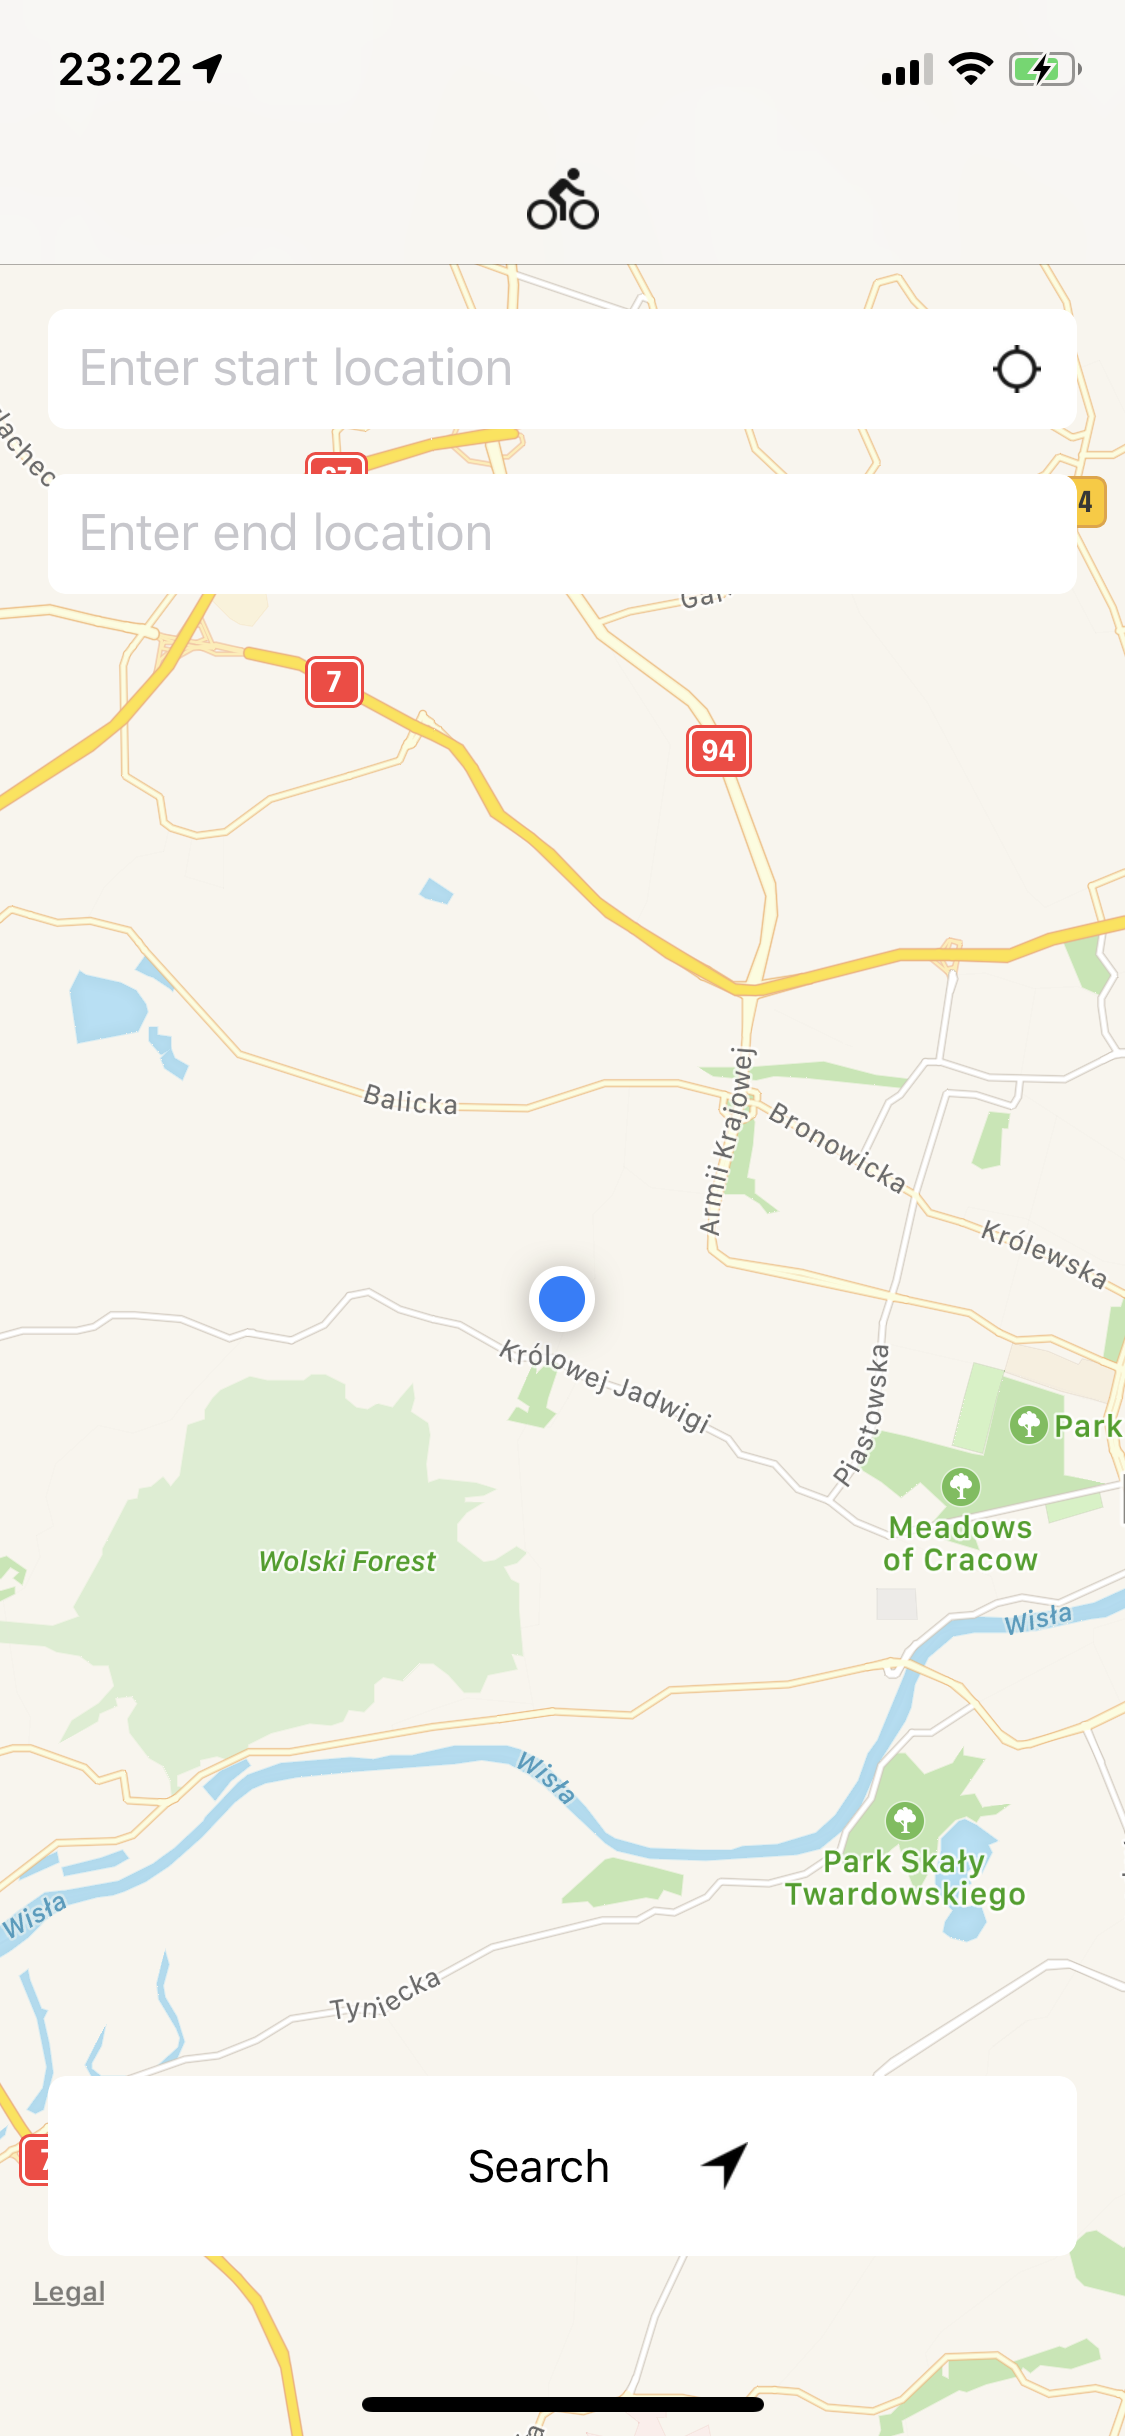
\includegraphics[height=9cm]{navi_initial}
\caption{Ekran początkowy aplikacji z możliwością wpisania punktów startowego i końcowego.}
\end{figure}

Po wprowadzeniu punktów końcowych trasy, następuje jej wyszukanie, w tym celu aplikacja przygotowuje zapytanie pod endpoint „findOptimized”, przekazując dane wpisane w polach tekstowych, a na czas ładowania odpowiedzi wyświetla indykator ładowania na górnym panelu oraz blokuje interakcje użytkownika ze wszystkimi elementami interfejsu poza mapą. Po pobraniu trasy jest ona przekształcana na modele po stronie aplikacji oraz rysowana na mapie. Linią ciągłą zaznaczona jest trasa, linią przerywaną odcinki poza trasą, które trzeba pokonać, aby dostać się z aktualnej lokalizacji użytkownika do początku trasy oraz z końca trasy do punktu końcowego wprowadzonego przez użytkownika. W celu wizualizacji, po narysowaniu mapa jest odpowiednio przybliżana tak, aby zaprezentować użytkownikowi przebieg całej trasy od jej początku do końca. Ekran z narysowaną mapą przedstawiono na poniższej ilustracji.

\begin{figure}[H]
	\begin{center}
		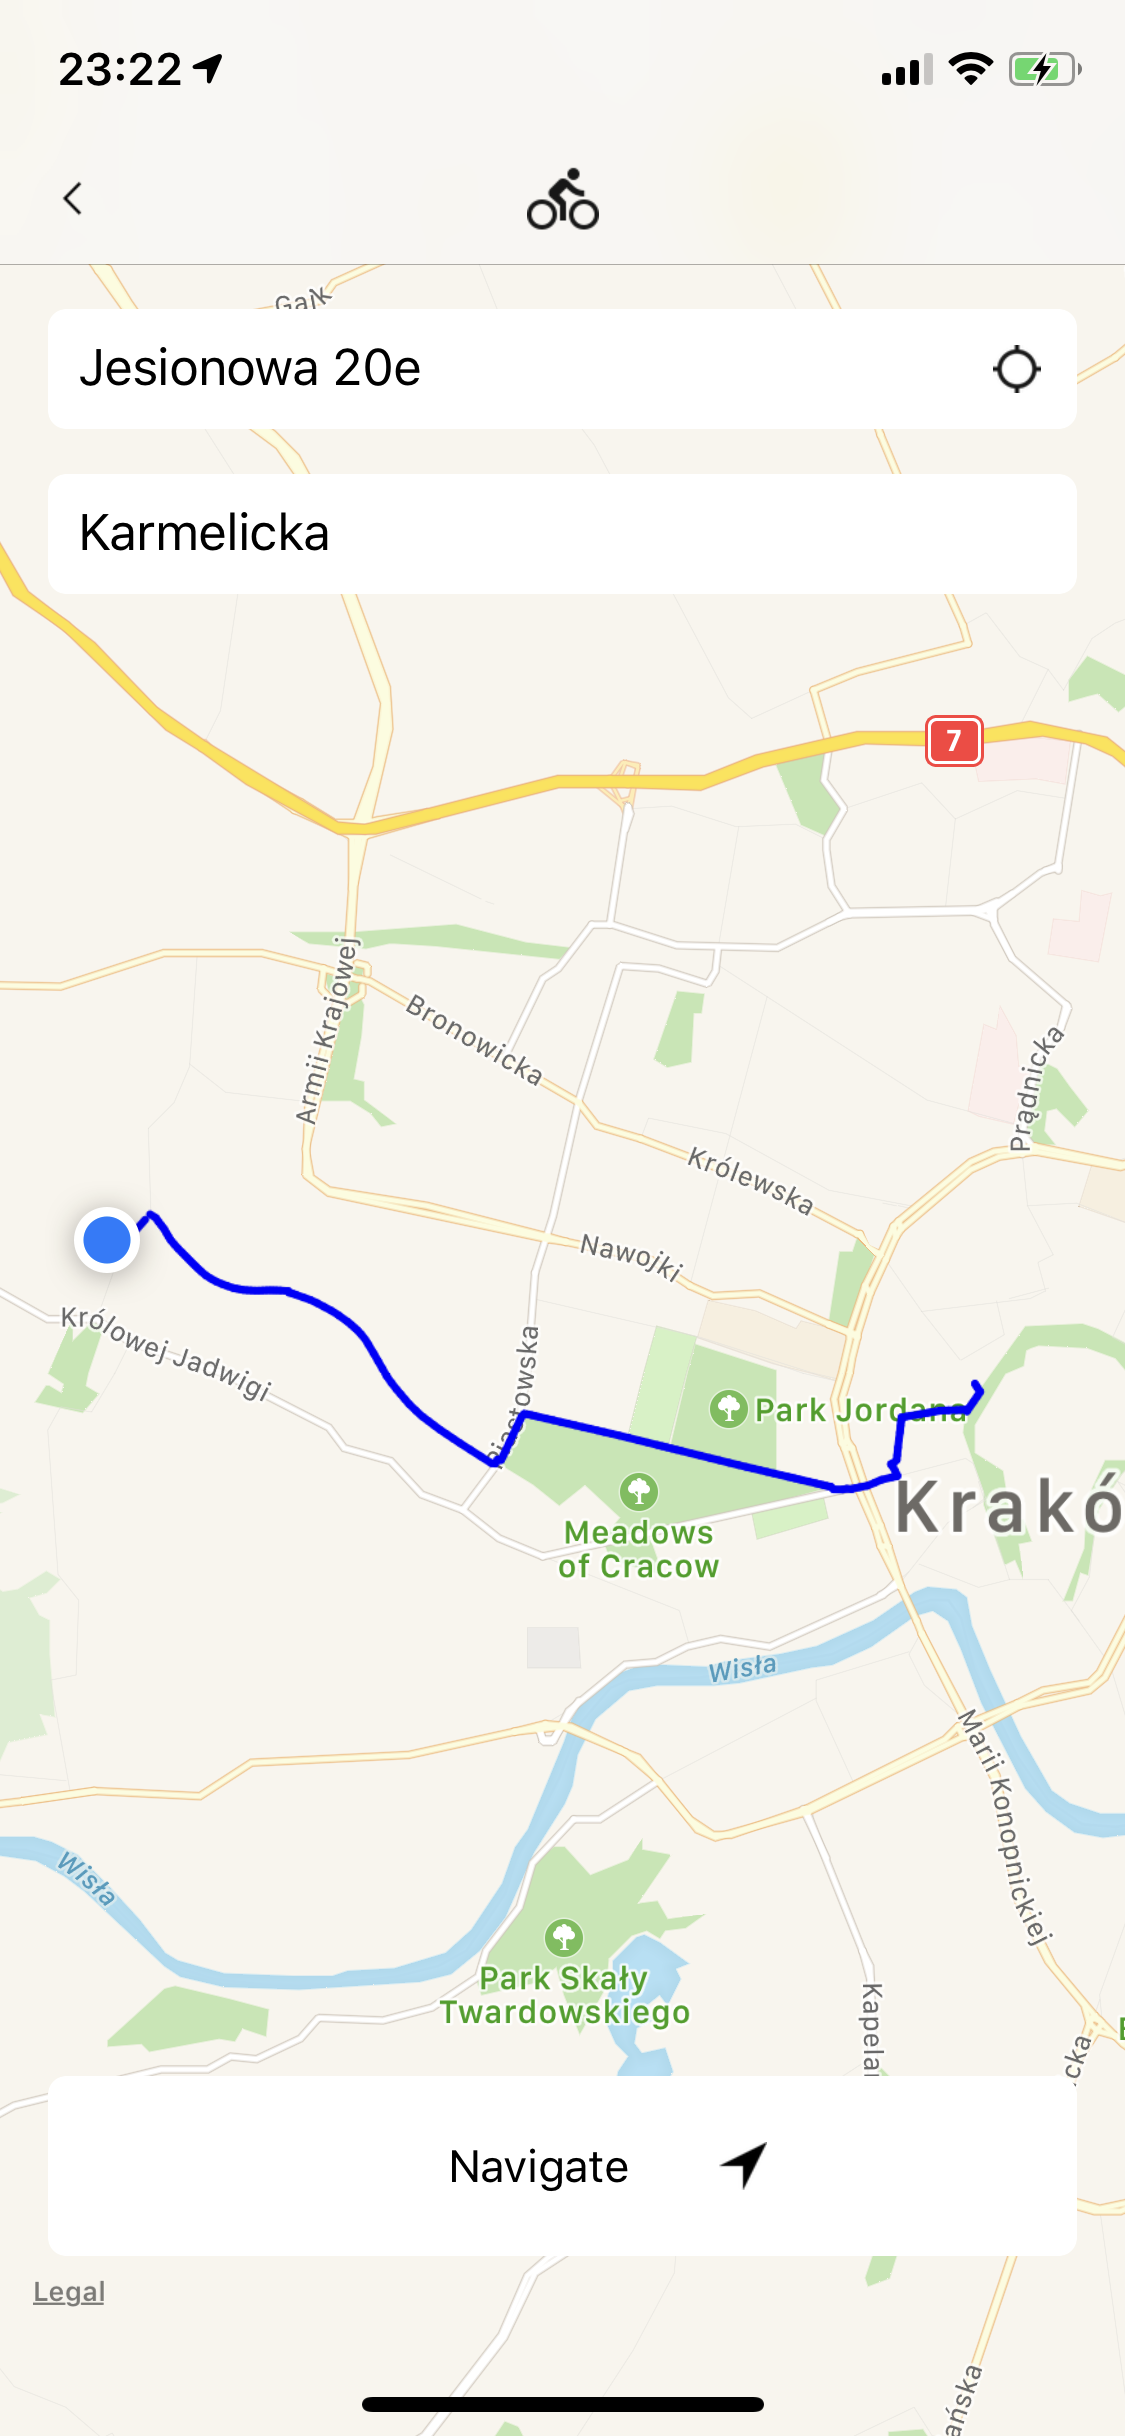
\includegraphics[height=9cm]{navi_route_marked}
	\end{center}
	\caption{Ekran aplikacji mobilnej podczas prezentacji wyznaczonej trasy.}
\end{figure}

Po wciśnięciu przycisku "nawiguj" zostaje włączony proces nawigacji użytkownika po trasie. W pierwszej fazie jest to prowadzenie do początku trasy. Mapa zostaje odpowiednio przybliżona, aby objąć drogę z aktualnego położenia użytkownika do początku trasy. Lokalizacja użytkownika jest przedstawiona w postaci standardowego punktu na mapie, obsługiwanego przez bibliotekę MapKit.

\begin{figure}[H]
\centering
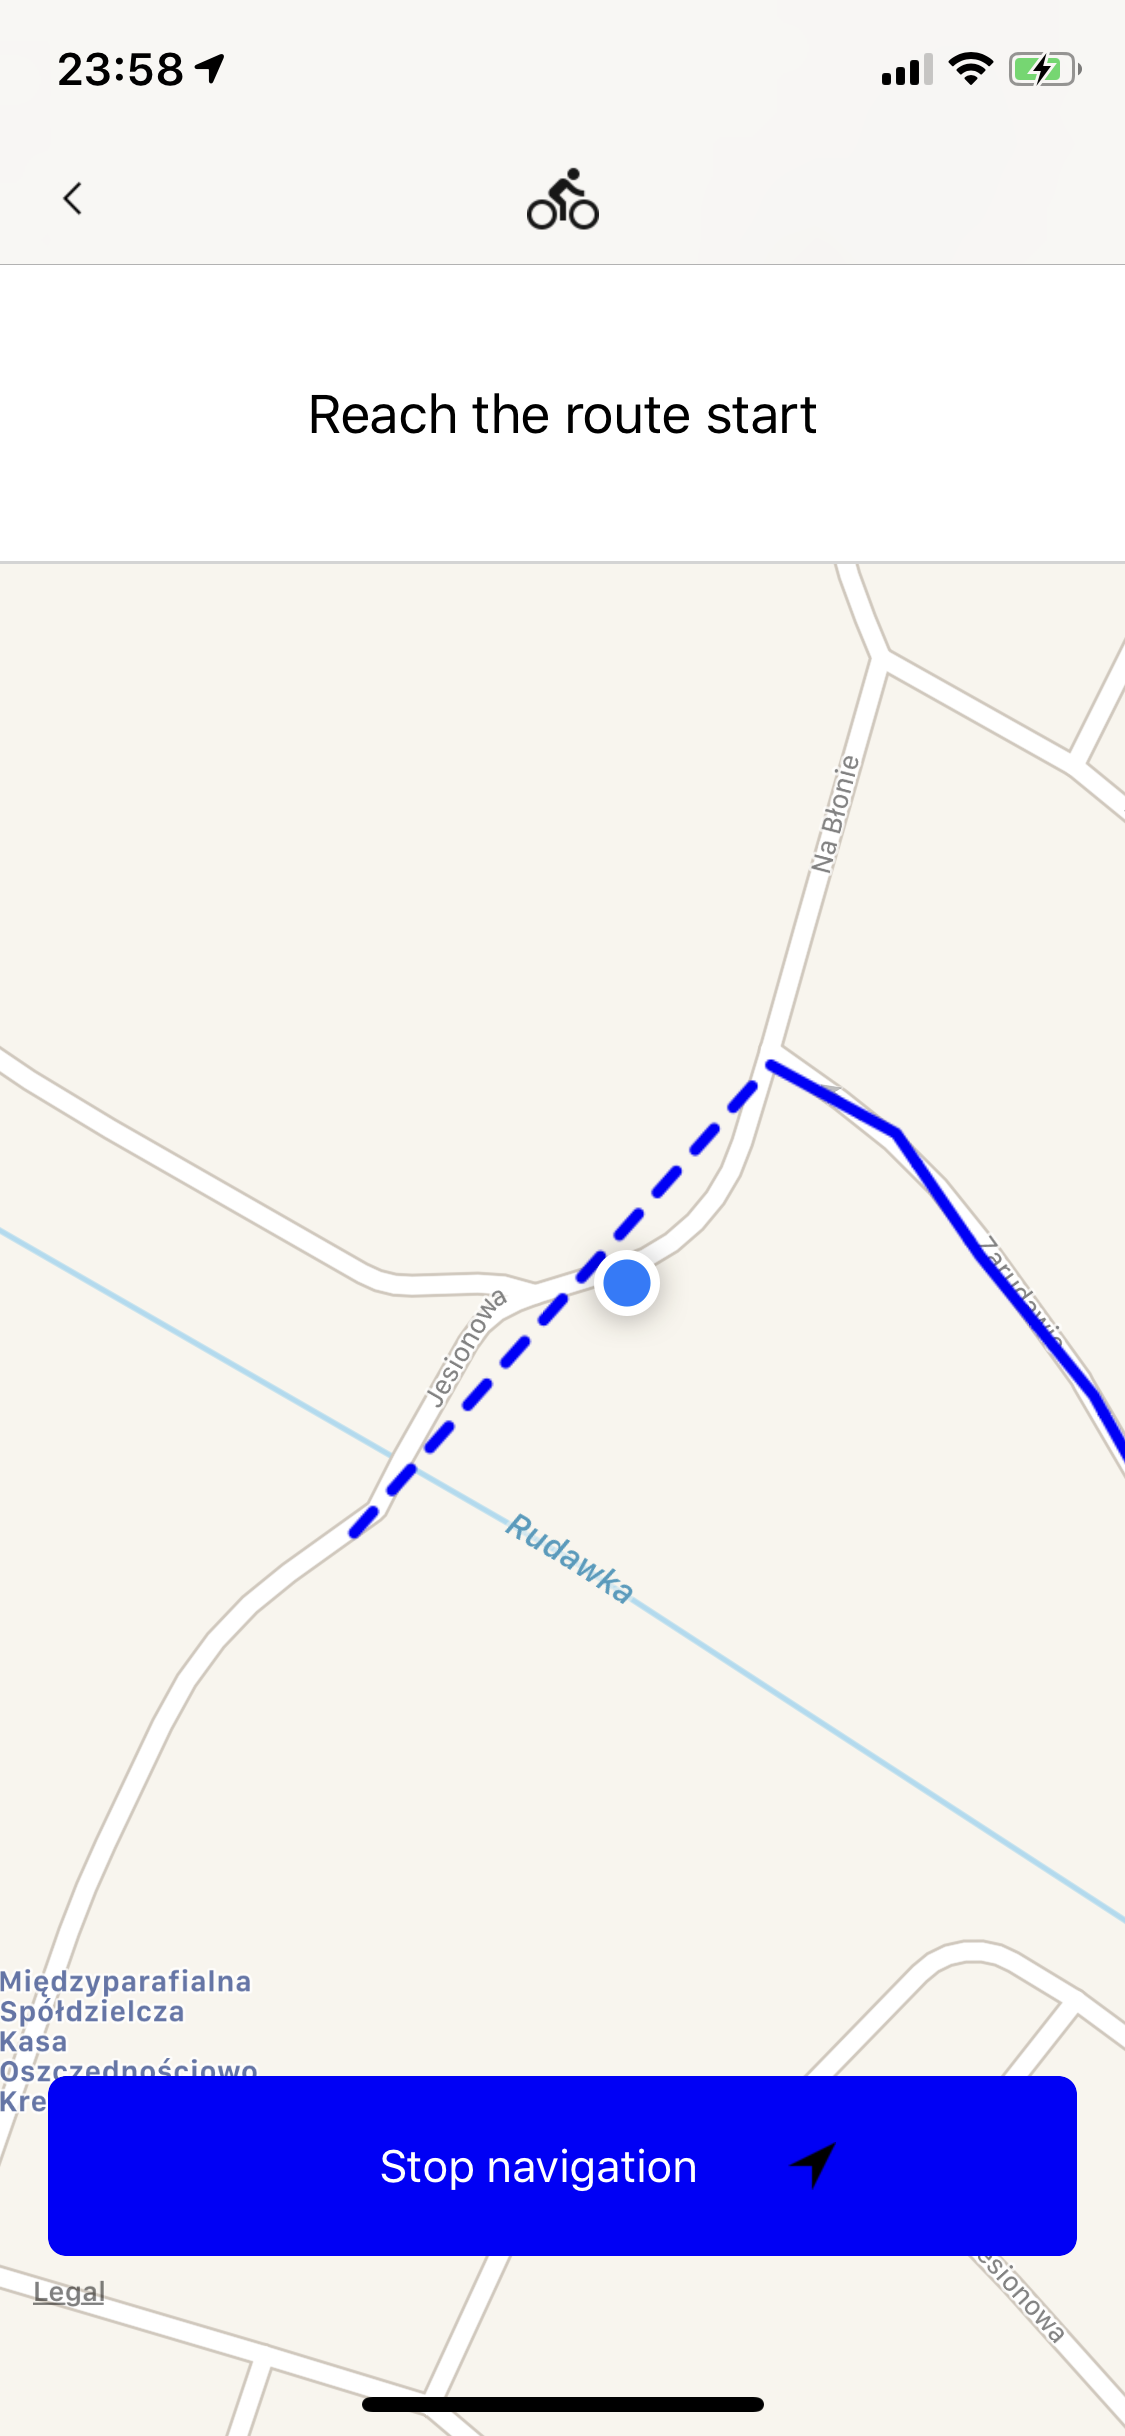
\includegraphics[height=9cm]{navi_reach_start}
\caption{Ekran aplikacji mobilnej w stanie, w którym użytkownik ma za zadanie dotrzeć do początku trasy.}
\end{figure}

Po dojściu użytkownika w obręb wyznaczonej trasy, interfejs aplikacji rozpoczyna nawigowanie go po trasie. Punkt wyznaczający aktualną lokalizację jest co sekundę animowanie przesuwany na pozycję na trasie, odpowiadającą najbliższemu segmentowi w stosunku do rzeczywistej pozycji użytkownika na mapie. W przypadku wykrycia przez aplikację zakrętu w zasięgu około najbliższych 200 metrów, na górnym panelu jest wyświetlana wskazówka zawierająca kierunek zakrętu oraz aktualną odległość po której wystąpi. W przypadku, gdy użytkownik zjedzie z trasy, na górnym panelu jest przedstawiona instrukcja sugerująca powrót na trasę, zaś gdy oddali się od niej za daleko, instrukcja zmienia się w informację o wyznaczaniu nowej trasy do punktu końcowego.

\begin{figure}[H]
\centering
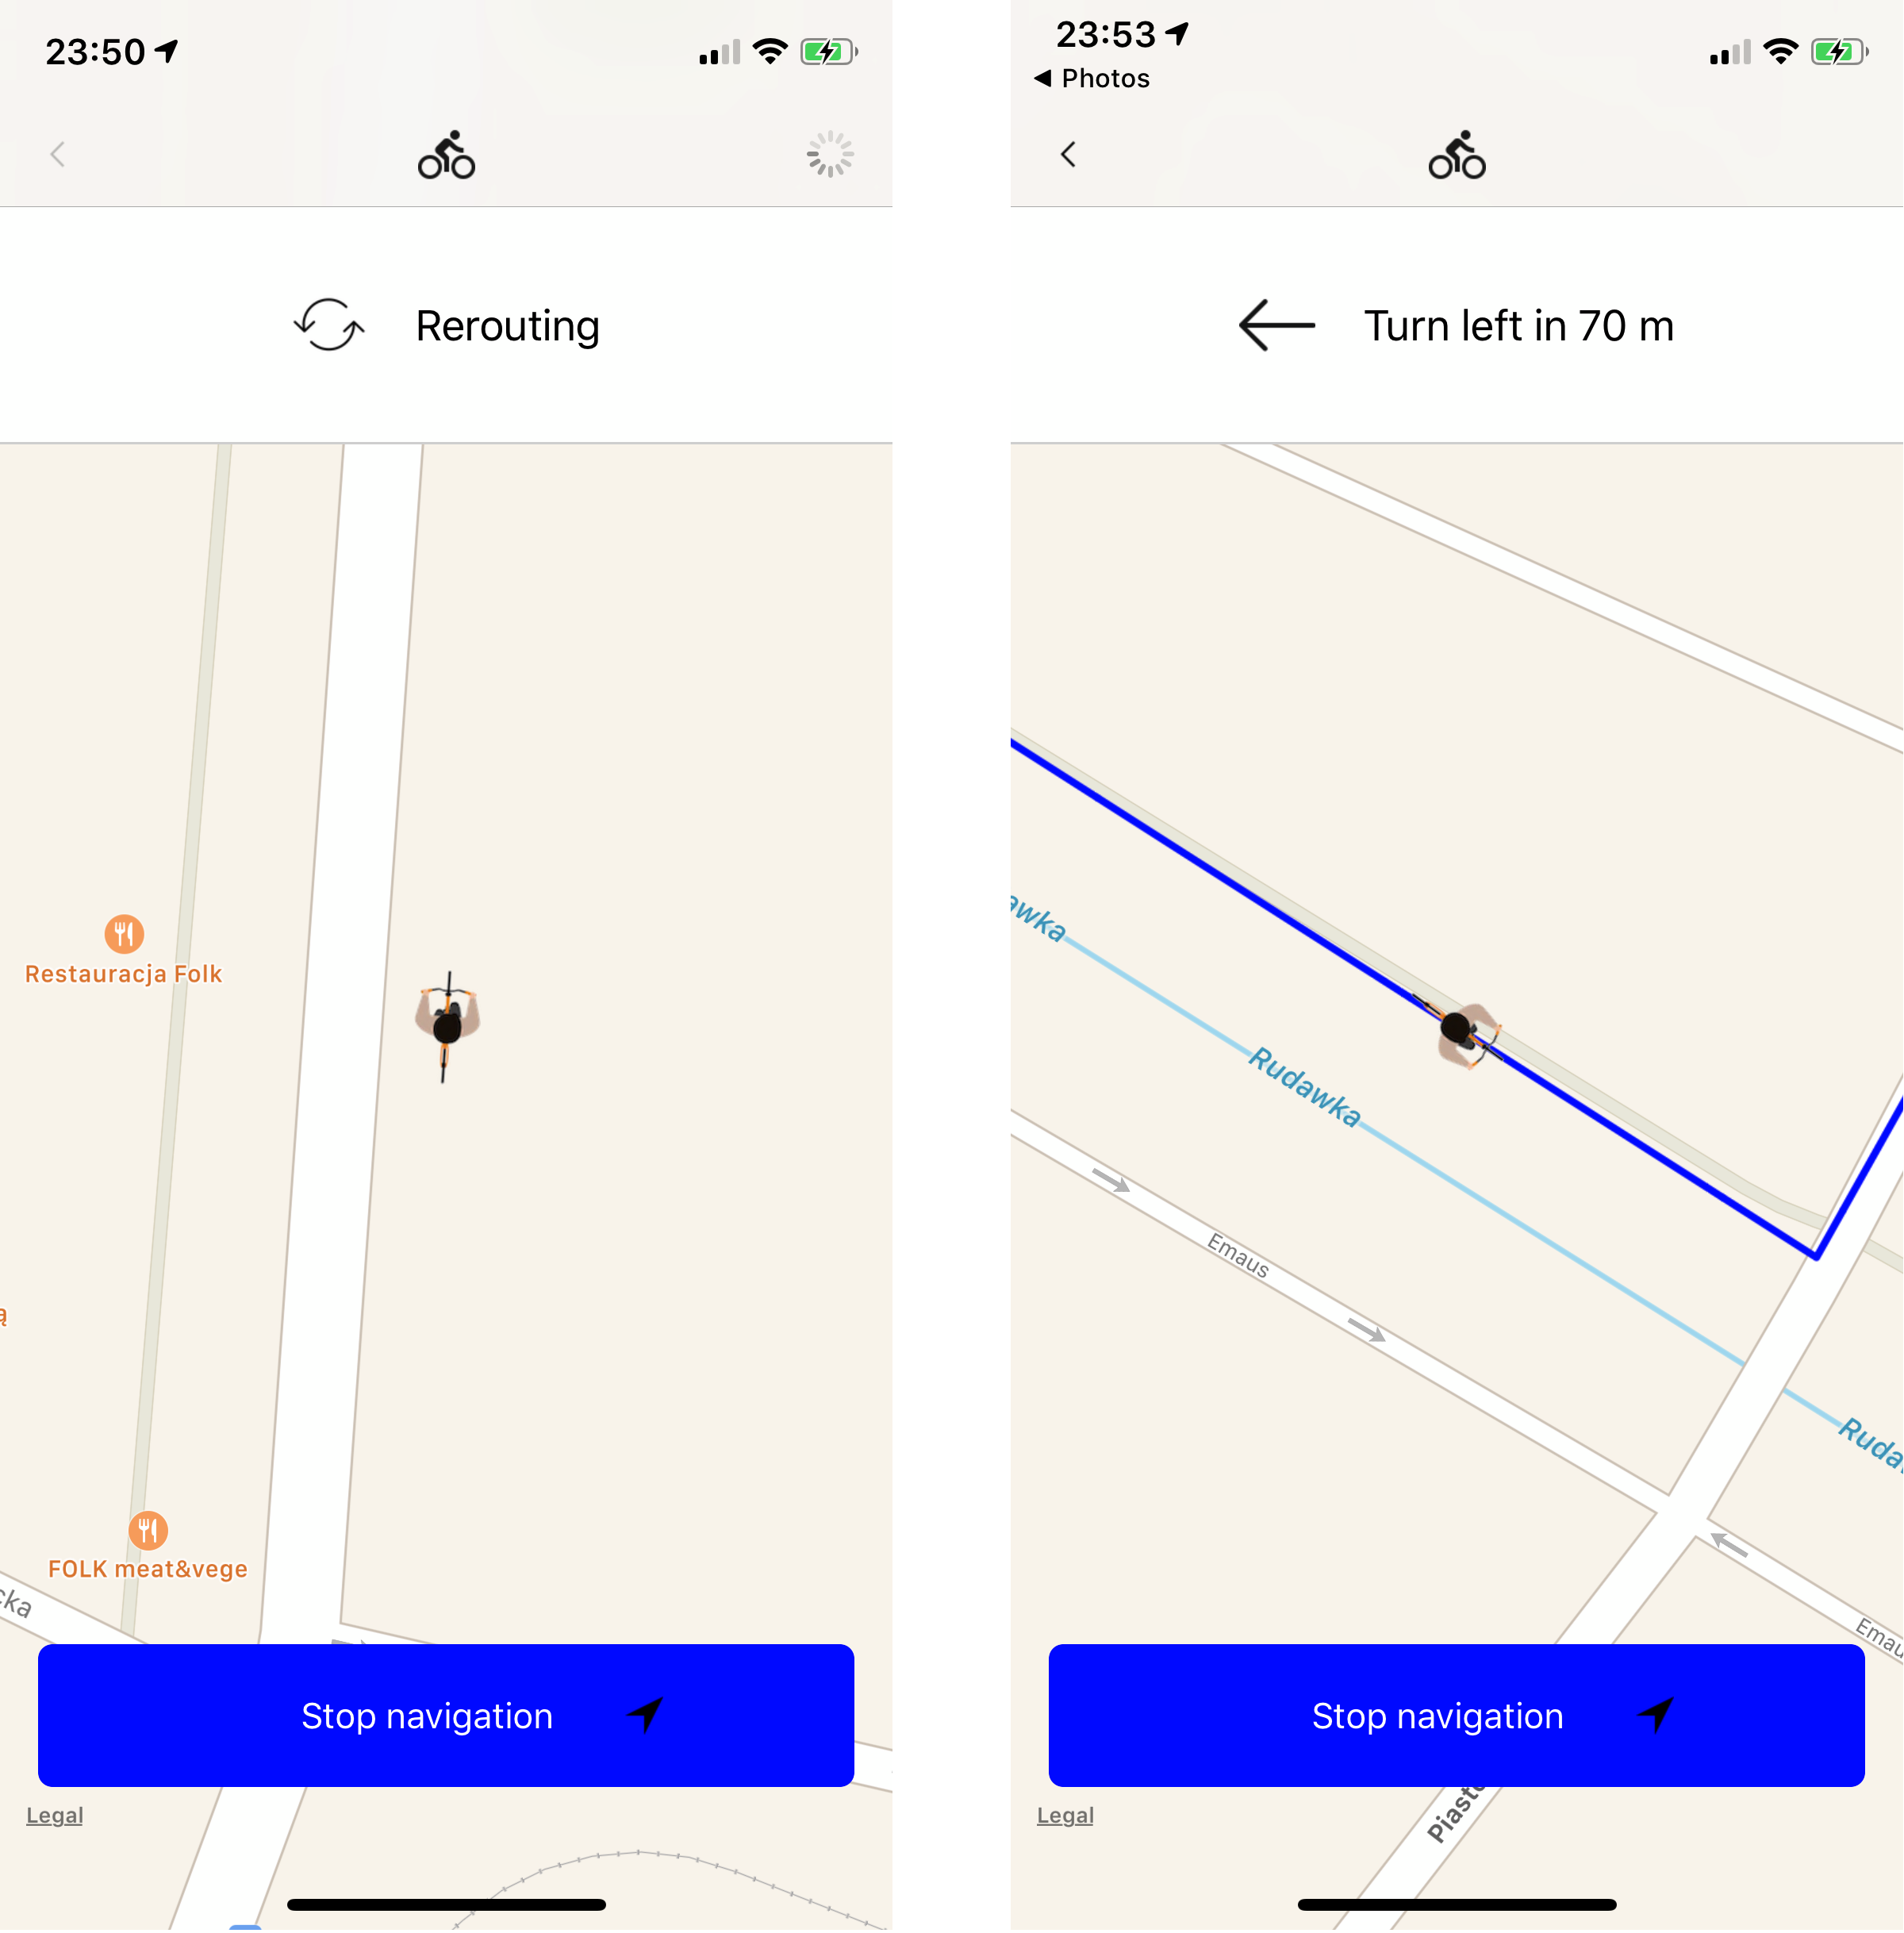
\includegraphics[height=9cm]{navi_guidance}
\caption{Ekrany aplikacji mobilnej przedstawiające wskazówki nawigacji podczas poruszania się po trasie.}
\end{figure}

\subsection{Opis działania nawigacji}

System nawigacji w aplikacji został zaimplementowany w celu wizualizacji aktualnej lokalizacji użytkownika w stosunku do trasy, która została wyznaczona. Działanie systemu składa się z zestawu stanów pomiędzy, którymi algorytm może przechodzić w przypadku wykrycia określonych warunków. W poniższym akapicie została przedstawiona lista stanów, na które składa się proces nawigacji, a także dokładny opis warunków koniecznych do przejścia pomiędzy nimi. W celu wizualizacji procesu został także stworzony diagram stanów odwzorowujący cały proces.

Lista stanów, w których może znaleźć się proces nawigacji użytkownika:

\begin{itemize}
\item Dotarcie z aktualnej lokalizacji do punktu startowego trasy
\item Nawigacja użytkownika po trasie
\item Dotarcie z końca trasy do punktu końcowego nawigacji
\item Zejście z trasy - w przypadku, gdy użytkownik znalazł się w odległości większej niż 30m, ale nie większej niż 150m od trasy.
\item Potrzeba wyznaczenia nowej trasy - gdy użytkownik znalazł się w odległości większej niż 150m od najbliższego segmentu trasy.
\end{itemize}

W momencie, gdy użytkownik rozpoczyna nawigację, zostaje włączony proces, który co sekundę pobiera aktualną lokalizację użytkownika z klienta lokalizacji i wyznacza aktualny stan aplikacji. Startowym stanem jest prowadzenie użytkownika do początku trasy. Jako, że pokrycie Krakowa drogami dla rowerów oraz drogami z niskim ograniczenie prędkości jest względnie małe, w większości przypadków użytkownik na początku będzie musiał przemieścić się kilkaset metrów poza trasami wspieranymi przez aplikację. W tym celu jest rysowana prosta linia pomiędzy punktem początkowym, wpisanym przez użytkownika, a początkiem trasy, a mapa jest odpowiednio przybliżana, aby umożliwić użytkownikowi proste dotarcie do drogi. \newline
W czasie fazy prowadzenia użytkownika na start trasy, co każdy cykl odświeżania aktualnego stanu, jest sprawdzane czy użytkownik znalazł się w otoczeniu 10 metrów w stosunku do początku któregokolwiek z segmentów składających się na trasę. Sprawdzanie jedynie segmentu będącego punktem początkowym trasy nie daje w tym wypadku oczekiwanego rezultatu ze względu na częste błędy w wyznaczeniu pozycji użytkownika przez moduł GPS, a także przez fakt, że często na trasę wjeżdżamy niedokładnie w punkcie jej początku, a przykładowo dopiero po pierwszych stu metrach. Posiadając dostępny zbiór danych aplikacja niestety nie jest w stanie wyznaczyć optymalnej drogi użytkownika pomiędzy jego aktualnym położeniem a punktem końcowym trasy. Jesteśmy w stanie jedynie oszacować, że najbardziej prawdopodobnym punktem będzie najbliższy wierzchołek grafu, zakładając odpowiednią granulację wszystkich wierzchołków otrzymanych podczas procesu jego tworzenia. \newline
W przypadku wykrycia wejścia użytkownika w obręb wyznaczonej dla niego trasy, aplikacja przechodzi w stan nawigowania po drodze. Aby uniknąć błędów w wyznaczaniu pozycji użytkownika i prowadzenia go w odległości 10-20 metrów obok zaznaczonej drogi, został zaimplementowany mechanizm "dociągania" do wyznaczonej ścieżki. W każdym kroku filtrowane są wszystkie drogi w celu znalezienia tej znajdującej się najbliżej użytkownika, zastosowano do tego porównanie sumy odległości od początków z każdej tych dróg, podzielonej przez jej długość. Dzięki temu rozwiązaniu algorytm wyeliminował znajdywanie jedynie krótkich dróg, dla których suma odległości do początku oraz do końca była najmniejsza. \newline
Po odnalezieniu najbliższej drogi, algorytm przeszukuje wszystkie jej segmenty w celu znalezienia tego znajdującego się najbliżej. Jako że długości segmentów zostały ujednolicone w jednym z kroków tworzenia grafu, na tym etapie możemy zastosować prostsze porównanie, które sprawdza jedynie sumę odległości użytkownika od początku oraz końca każdego z segmentów.
W następnym kroku, uzyskany segment zostaje podzielony na 20 równych sobie odcinków. Najbliższy aktualnej pozycji użytkownika zostaje przypisany jako najbardziej odpowiedni, a aplikacja sztucznie dociąga lokalizację użytkownika do tego właśnie punktu. \newline
Metoda opisana powyżej działa w przypadku, gdy wyznaczona pozycja użytkownika znajduje się nie dalej niż 50 metrów od trasy. W przypadku, gdy użytkownik znajdzie się w odległości większej niż 50 metrów, algorytm przestaje zwracać pozycję użytkownika dociągniętą do trasy, a zamiast tego zwraca rzeczywiste położenie użytkownika na mapie. Ten tryb został zaimplementowany w celu przedstawienia użytkownikowi informacji o tym, że znalazł się poza trasą i powinien na nią wrócić. Ogranicza to także niepotrzebne zapytania do strony serwerowej w przypadku, gdy użytkownik celowo zszedł z trasy, aby na przykład wejść do sklepu.
W przypadku, gdy wykryte położenie znajduje się dalej niż 150m od trasy zaznaczonej na mapie, algorytm zakłada, że należy dla użytkownika wyznaczyć nową trasę, o czym informuje przez wysłanie określonego sygnału oraz zakończenie działania. W tym momencie zostaje wysłane zapytanie do serwera o nową trasę zawierające aktualną pozycję użytkownika oraz miejsce docelowe określone na początku procesu nawigacji. W przypadku gdy zapytanie się powiedzie, algorytm zostaje zrestartowany i wraca do stanu początkowego, czyli prowadzenia użytkownika do początku trasy. \newline
W każdym kroku działania algorytmu jest także sprawdzana odległość aktualnej pozycji użytkownika od końca wyznaczonej trasy. Jeśli jest ona mniejsza niż 50 metrów, zakładamy, że użytkownik dotarł do końca i nawigacja przechodzi w tryb prowadzenia użytkownika do punktu końcowego trasy, pokazując jednocześnie odpowiednio przybliżony obszar na mapie. W tym kroku założona odległość od punktu końcowego musi być znacznie większa niż ta która stanowi o momencie wejścia na trasę, ponieważ użytkownik może znajdywać się w najbliższym otoczeniu punktu końcowego jedynie przez krótką chwilę.


\subsection{Opis testów}

Do testów działania nawigacji zostały wykorzystane pliki GPX (\textit{GPS Exchange Format}), które sformatowane w odpowiedni sposób umożliwiają symulację lokalizacji użytkownika zarówno przy użyciu symulatora, jak i na rzeczywistym urządzeniu z systemem iOS. Plik GPX jest to plik w formacie XML, który składa się ze zbioru punktów oraz czasów skorelowanych z każdym z nich. System odczytując ten plik animuje lokalizację użytkownika tak, aby przeszła ona pomiędzy wszystkimi określonymi punktami w ściśle wyznaczonym czasie. Do stworzenia plików użyto strony \textit{http://www.gpsies.com/createTrack.do} która udostępnia graficzny interfejs do zaznaczania punktów na mapie oraz określenia z jaką prędkością chcielibyśmy, aby użytkownik się pomiędzy nimi przemieszczał. Pobrany stamtąd plik następnie trzeba poddać obróbce w postaci usunięcia kilku linii, aby był wspierany przez symulację lokalizacji w systemie iOS.

\section{Opis stworzonej strony internetowej}

\subsection{Opis technologii i użytych bibliotek}

W ramach projektu została zaimplementowana także strona internetowa, która w intuicyjny sposób pozwala użytkownikowi wyszukać trasę pomiędzy wpisanymi adresami oraz wyświetla ją na mapie. 
Aplikacja została stworzona w oparciu o bibliotekę ReactJS, która pozwala w szybki sposób zbudować prototyp strony internetowej przy użyciu języka Javascript oraz predefiniowanych elementów strony, takich jak przyciski czy pola tekstowe. Do wyświetlenia map użyto map udostępnionych przez \textit{openstreetmap} używając biblioteki React Leaflet. Leaflet jest to biblioteka umożliwiająca bardzo proste renderowanie map przy użyciu Javascript, React Leaflet dodaje do tego mapy w postacie gotowych komponentów React. Wybór został podyktowany faktem, że prostsze w użyciu i wydajniejsze mapy Google, w celu wyświetlenia przy użyciu języka Javascript, wymagają płatnej subskrybcji.
W projekcie strony internetowej, do zarządzania zewnętrznymi zależnościami, użyto programu yarn, a do zapytań http użyto biblioteki axios. Narzędzia te nie różnią się od tych dla aplikacji serwerowej, dlatego też w tym akapicie pominięto ich opis.

\subsection{Spis ekranów, opis działania}

Aplikacja jest nieskomplikowana, składa się z dwóch ekranów. Na pierwszym z nich są przedstawione dwa pola tekstowe oraz przycisk umożliwiający wyszukanie trasy. Jej wygląd przedstawiono na poniższej ilustracji.

\begin{figure}[H]
\centering
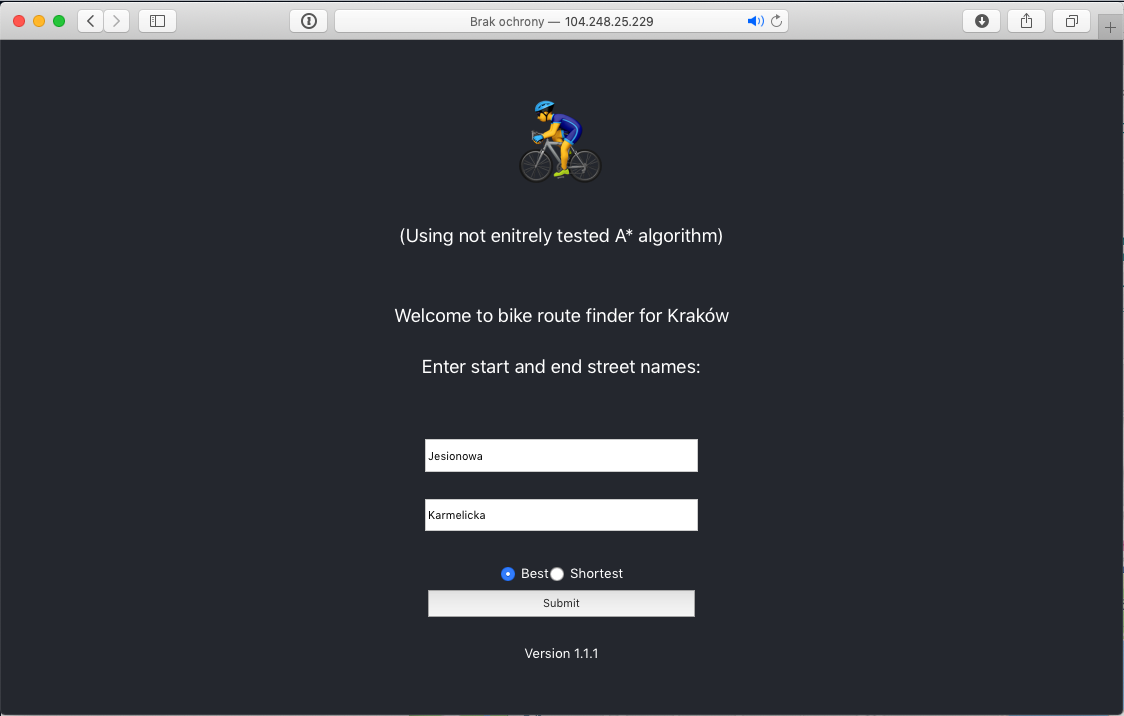
\includegraphics[width=\textwidth]{web_form}
\caption{Ekran domowy strony internetowej.}
\end{figure}

Kolejny z ekranów ma zaimplementowaną logikę pobierania trasy w zależności od stanu przekazanego do niego z ekranu wpisywania danych. Wykorzystując bibliotekę axios wykonuje zapytanie pod endpoint „visualizationPoints” zawierając w kwerendzie wymagane dane. Zwrócona odpowiedź w formacie JSON zawiera zbiór wszystkich punktów na mapie, które należy ze sobą połączyć, aby przedstawić użytkownikowi wizualizację wyznaczonej ścieżki. Ścieżka przedstawiona jest na mapie obejmującej całość ekranu.

\begin{figure}[H]
\centering
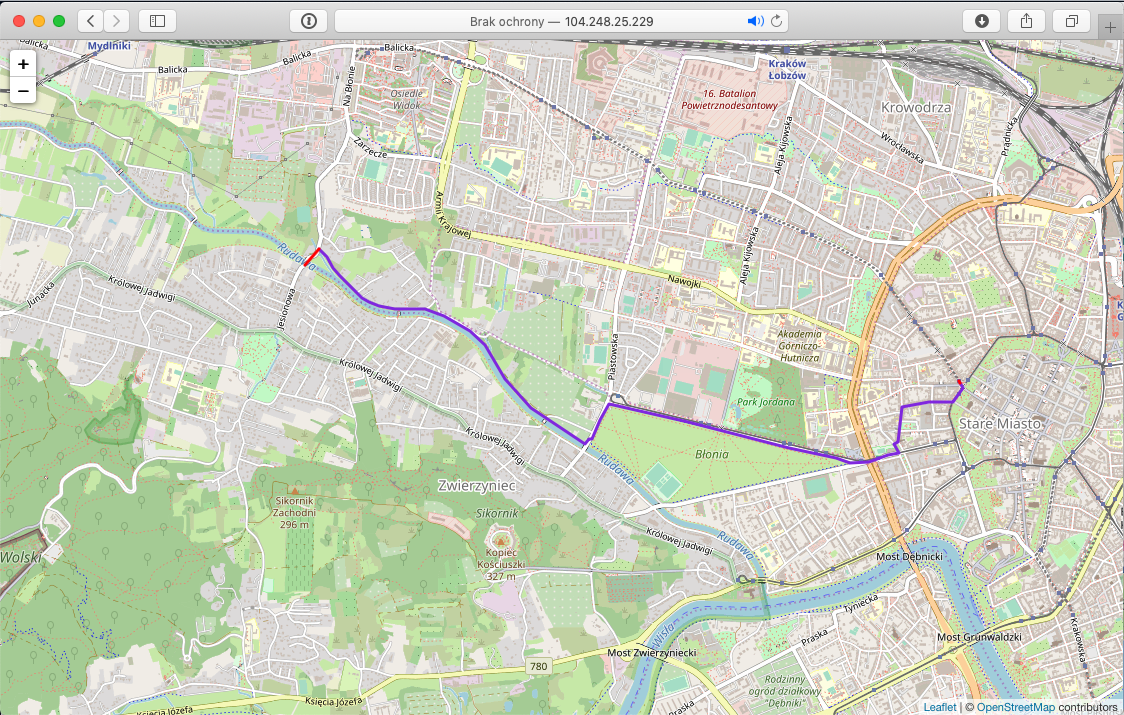
\includegraphics[width=\textwidth]{web_map}
\caption{Ekran strony internetowej z zaznaczoną trasą.}
\end{figure}
